\section{実ロボットを用いた実験}
実ロボットを用いて, 提案するシステムにより, ロボットが目的地へ到達可能であるか検証する.
\subsection{実験装置}
実験ではロボットを\ref{fig:gamma}に示す.ロボットはicart-miniをベースに本研究室で開発した
orne gammaを用いる.単眼のウェブカメラを3つ,
2D-LiDAR[(北陽電機 UTM-30LX)]を1つ搭載している. 
制御用の PC には GALLERIA GCR2070RGF-QC-Gを使用している.
メトリックマップベースのナビゲーションには,本学でNavigation stackをもとに開発した
orne navigationを使用する

% \begin{figure}[htbp]
%     \centering
%      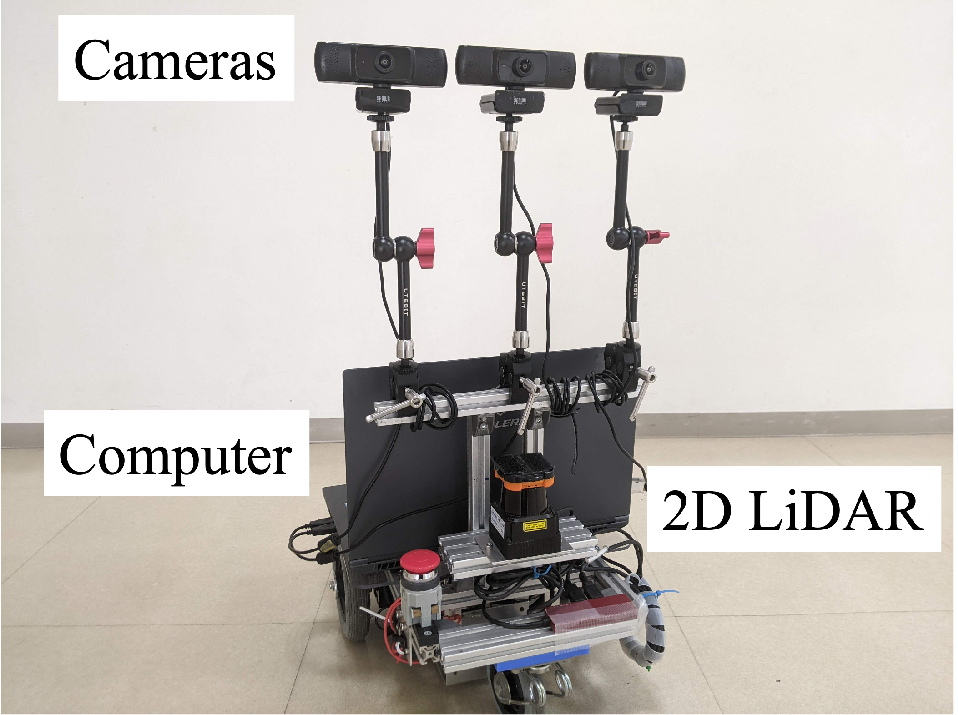
\includegraphics[width=100mm]{images/pdf/gamma_sensor.pdf}
%      \caption{Experimental setup}\label{fig:gamma}
% \end{figure}
\subsection{実験方法}
実験環境として\ref{fig:cit3f}に示す千葉工業大学津田沼キャンパス2号館3階の廊下を用いる.
環境中には,三叉路が4つ,角が2つ,突き当たりが2つ含まれている.
経路追従モジュールの訓練および通路分類モジュールのデータセット収集では
〜で示したaからnの経路を順番に走行する.
実験では島田らが用いた50例のシナリオの中から,
〜に示す7例を用いた.
選定の基準は,〜の場所を対象としていること.
ロボットが移動困難な狭い通路が含まれていないこと.
「後ろを向く」など経路追従モジュールができない行動が含まれていないことである.
% \begin{figure}[htbp]
%     \centering
%      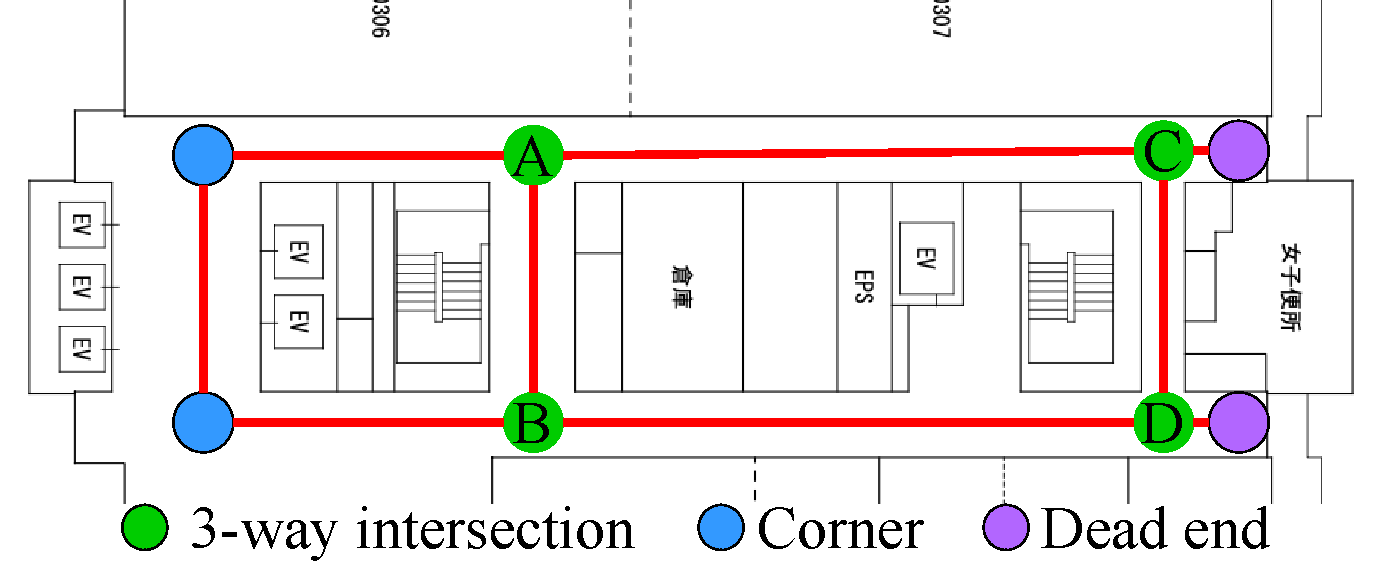
\includegraphics[width=100mm]{images/pdf/cit3f.pdf}
%      \caption{Experimental environment}\label{fig:cit3f}
% \end{figure}
% \begin{figure*}[htbp]
%     \centering
%      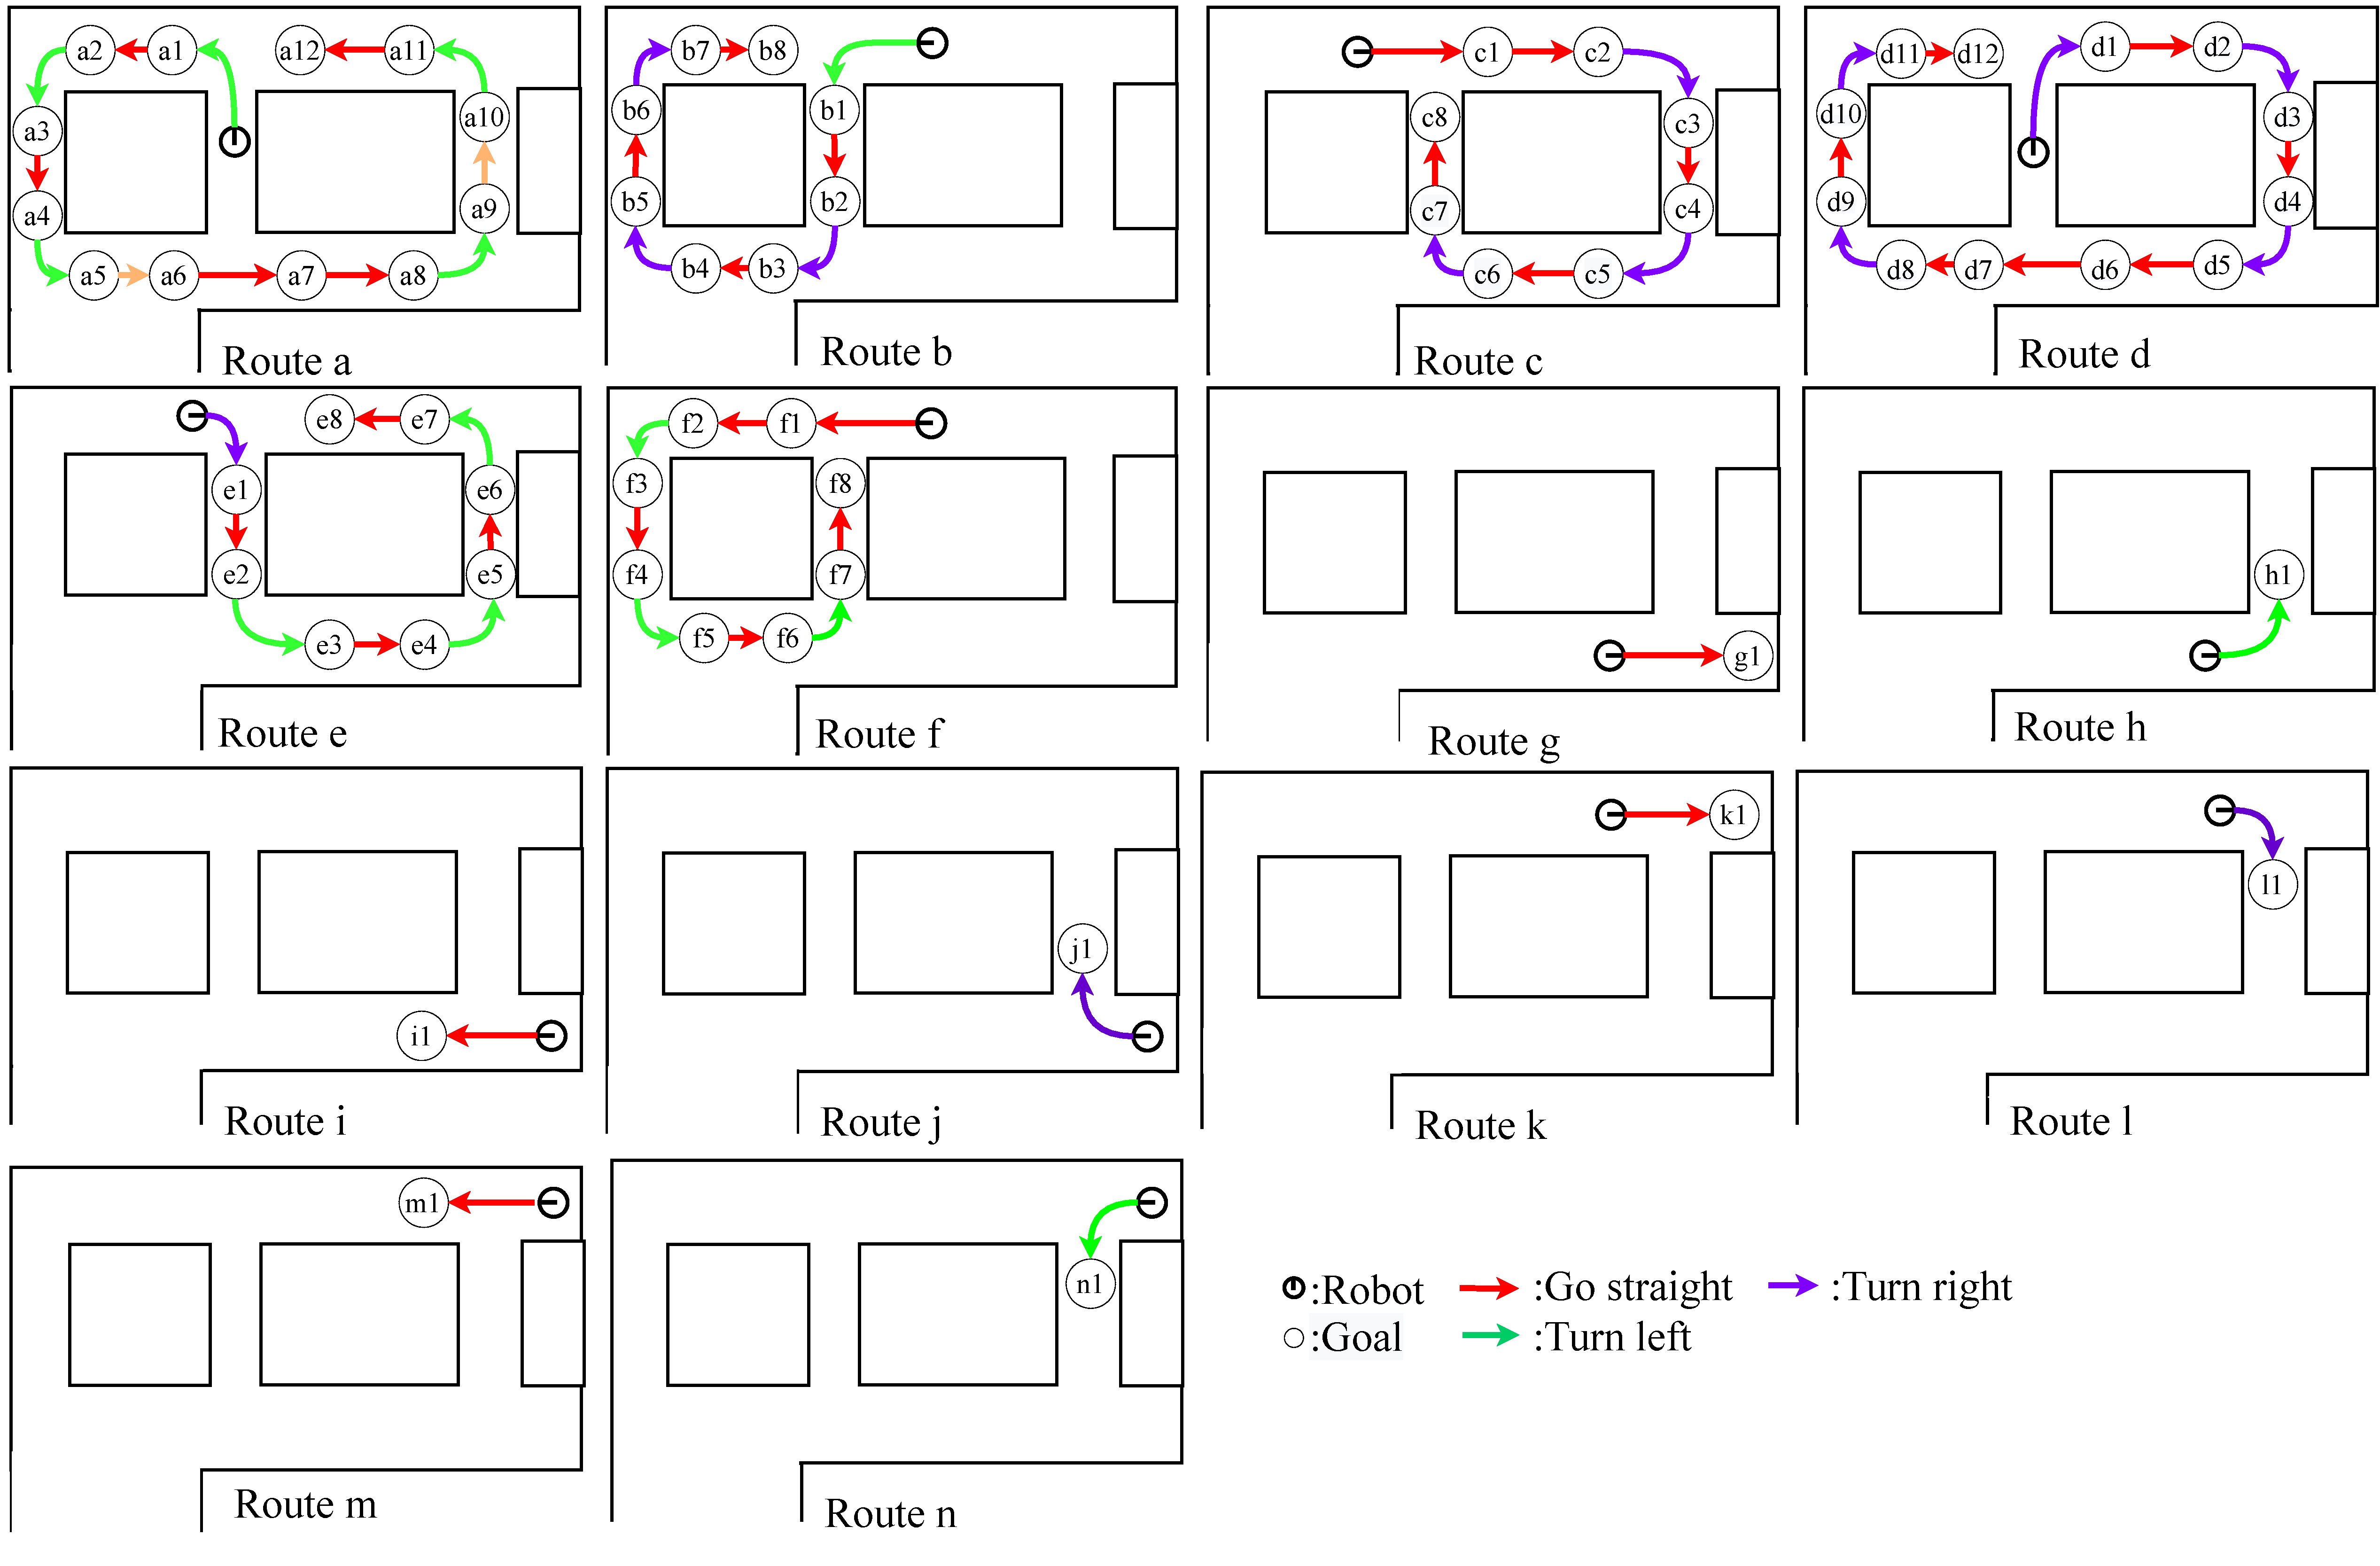
\includegraphics[width=120mm]{images/pdf/newroute.pdf}
%      \caption{Route used for learning}\label{fig:newroute}
% \end{figure*}
% \begin{figure*}[htbp]
%     \begin{tabular}{ccc}
%         \begin{minipage}[t]{0.3\textwidth}
%             \centering
%             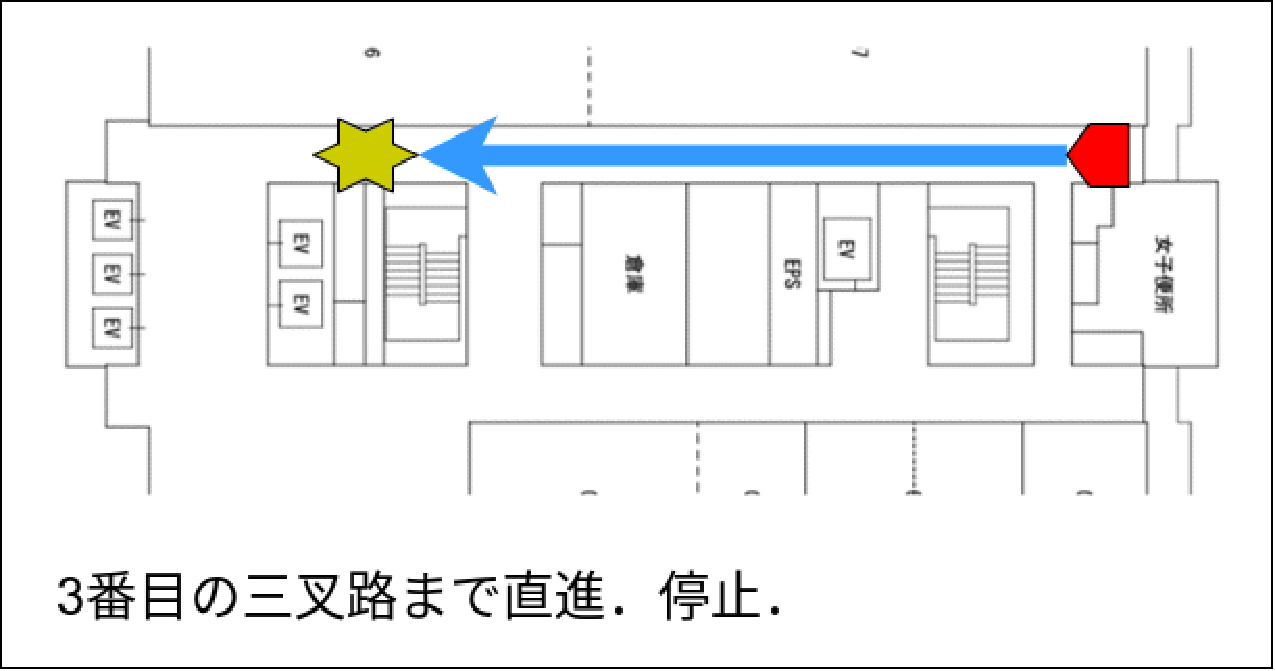
\includegraphics[keepaspectratio, width=57mm]{images/pdf/scenario/scenario01.pdf}
%             \subcaption{Scenario 01}
%             \label{composite}
%         \end{minipage} &
%         \begin{minipage}[t]{0.3\textwidth}
%             \centering
%             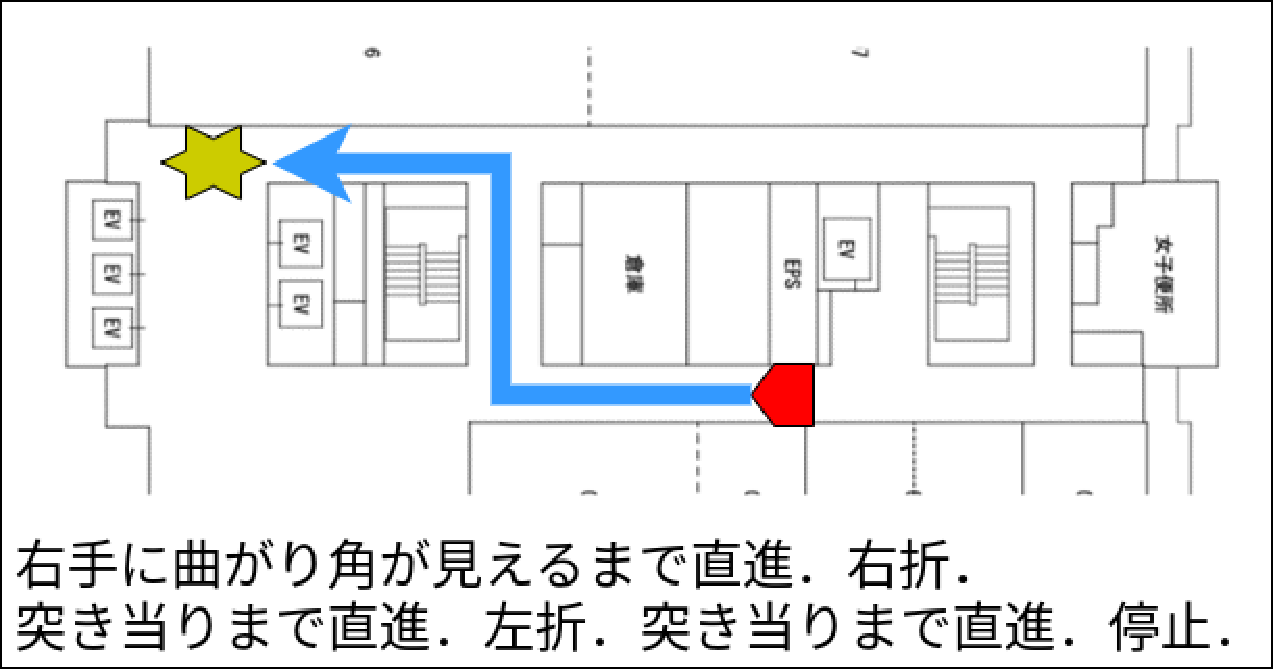
\includegraphics[keepaspectratio, width=57mm]{images/pdf/scenario/scenario02.pdf}
%             \subcaption{Scenario 02}
%             \label{Gradation}
%         \end{minipage} &
%         \begin{minipage}[t]{0.3\textwidth}
%             \centering
%             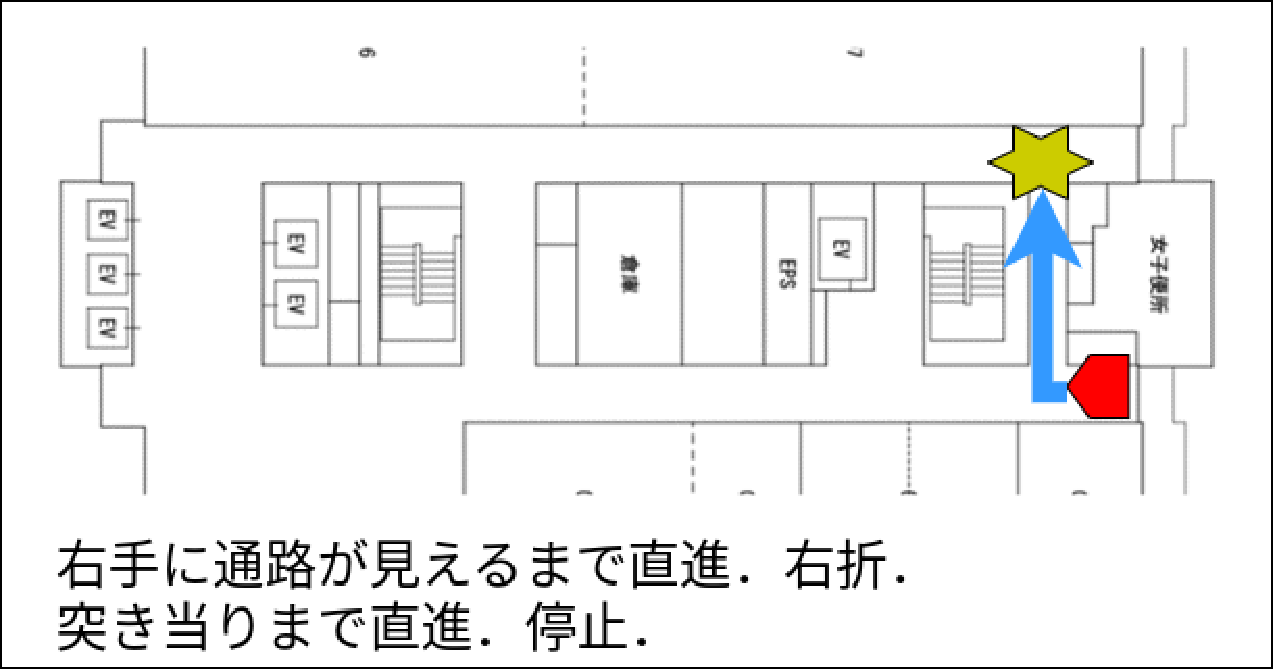
\includegraphics[keepaspectratio, width=57mm]{images/pdf/scenario/scenario03.pdf}
%             \subcaption{Scenario 03}
%             \label{fill}
%         \end{minipage} \\
%         \begin{minipage}[t]{0.3\textwidth}
%             \centering
%             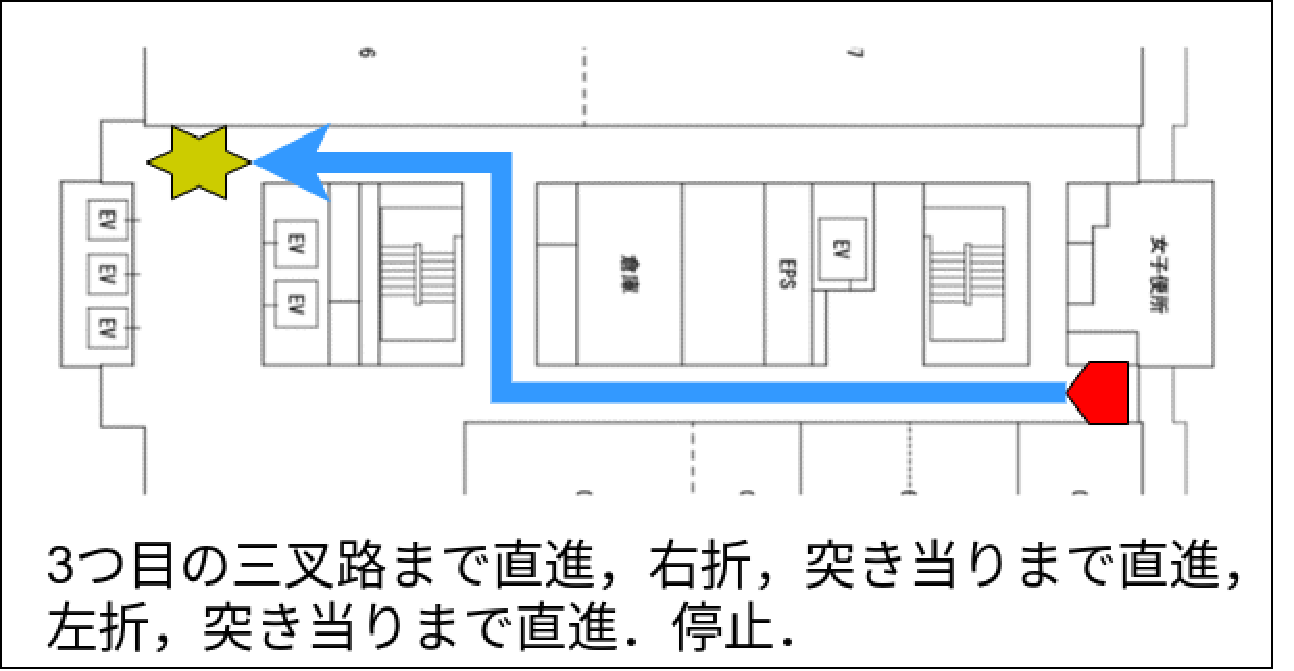
\includegraphics[keepaspectratio, width=57mm]{images/pdf/scenario/scenario04.pdf}
%             \subcaption{Scenario 04}
%             \label{transform}
%         \end{minipage} &
%         \begin{minipage}[t]{0.3\textwidth}
%             \centering
%             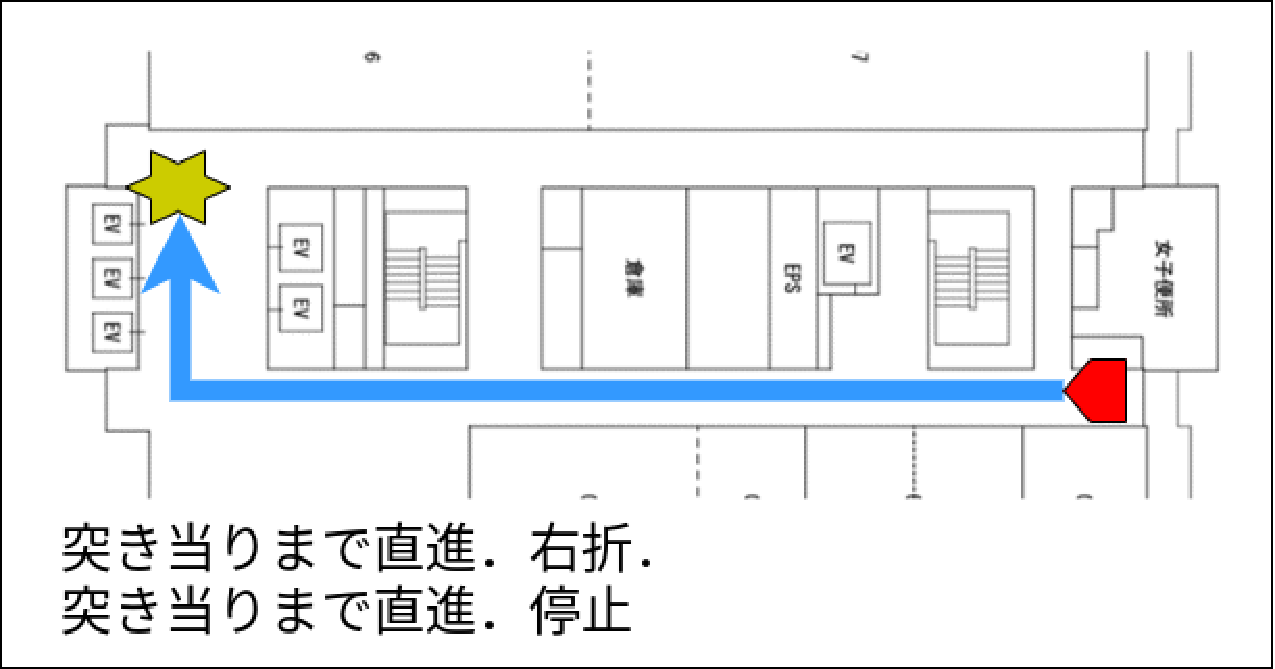
\includegraphics[keepaspectratio, width=57mm]{images/pdf/scenario/scenario05.pdf}
%             \subcaption{Scenario 05}
%             \label{image1}
%         \end{minipage} &
%         \begin{minipage}[t]{0.3\textwidth}
%             \centering
%             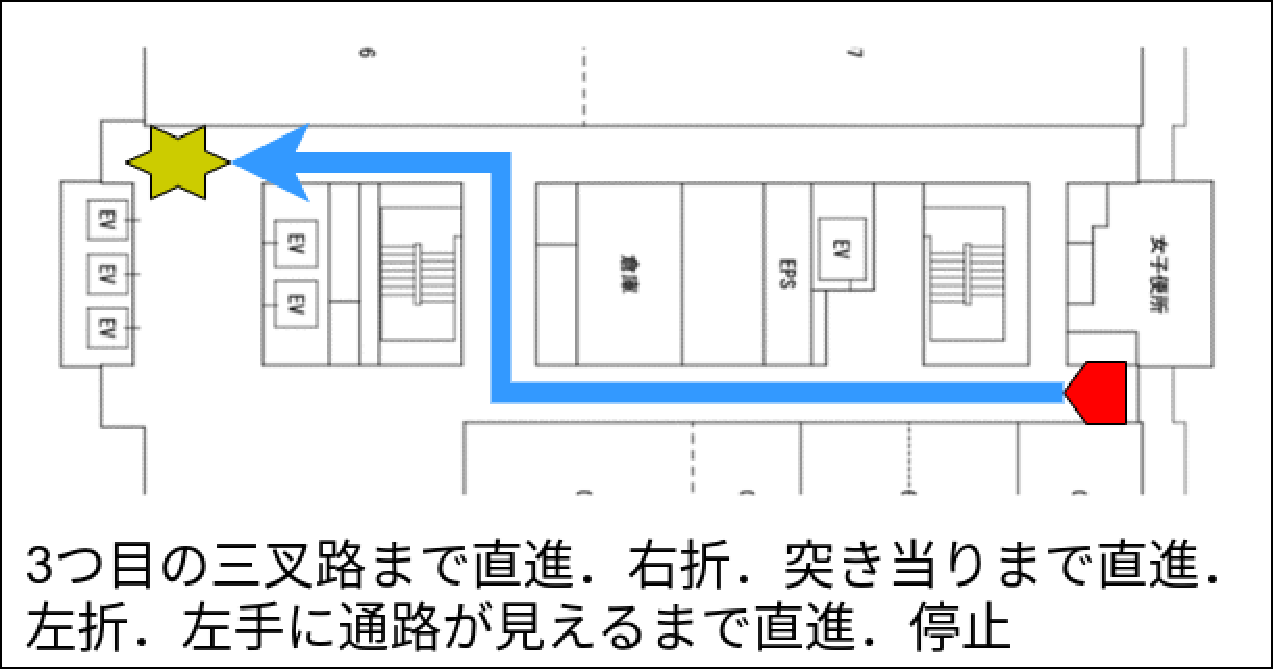
\includegraphics[keepaspectratio, width=57mm]{images/pdf/scenario/scenario06.pdf}
%             \subcaption{Scenario 06}
%             \label{fig:scenario24}
%         \end{minipage}\\
%         \begin{minipage}[t]{0.3\textwidth}
%             \centering
%             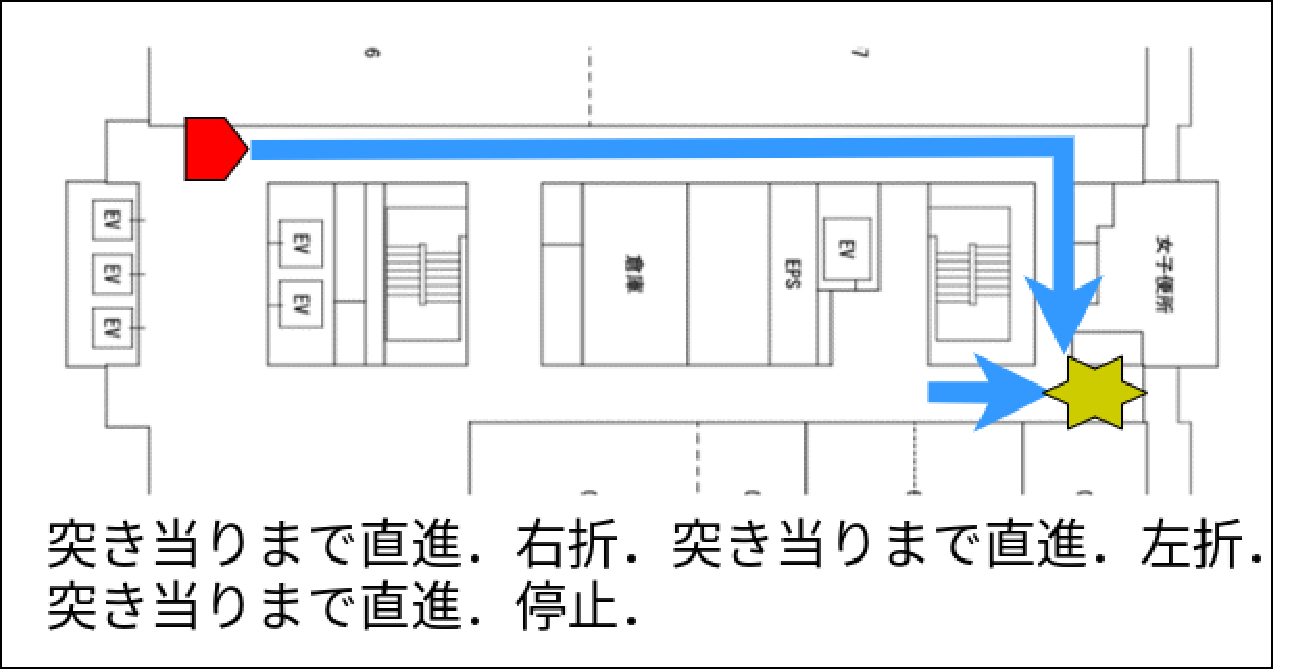
\includegraphics[keepaspectratio, width=57mm]{images/pdf/scenario/scenario07.pdf}
%             \subcaption{Scenario 07}
%             \label{imagess}
%         \end{minipage}
%     \end{tabular}
%     \caption{Scenarios used in the experiment}\label{fig:scenario_exp}
% \end{figure*}

\subsection{実験結果}
シナリオの道順に従い, 三叉路などの分岐路で適切に経路を選択して自律移動する
様子が見られた.結果として,7例すべてでロボットが, 目的地へ到達した.